%==============================================================
This chapter introduces an attempt to fabricate the 4004 CPU as actual silicon through the Tiny Tapeout.

%==============================================================
\section{Overview of the Tiny Tapeout}
%--------------------------------------------------------------
The current environment surrounding the semiconductor industry presents the following challenges:

\begin{itemize}
  \item Shortage of skilled personnel
  \item High development costs (tools, prototyping)
  \item Limited development opportunities
  \item Insufficient educational opportunities in semiconductors for children, students, and young engineers
  \item Difficulty in nurturing new talent
\end{itemize}

Against this backdrop, open-source semiconductors have recently attracted attention. This movement aims to open up and democratize semiconductor development, and rests on the following pillars:

\begin{itemize}
  \item Open-source EDA tools (free of charge)
  \item Open PDKs (free of charge and requiring no NDA)
  \item Low-cost shuttle prototyping services
\end{itemize}

As one embodiment of this movement, TinyTapeout has emerged as a service that allows even individuals to design and prototype IC chips (\url{https://tinytapeout.com/}). The supported manufacturing foundries include:

\begin{itemize}
  \item SkyWater (USA), 130\,nm
  \item IHP (Germany), 130\,nm
  \item GlobalFoundries (USA), 180\,nm
\end{itemize}

By using a shuttle-based approach that arranges multiple projects as tiles on a single chip for wafer fabrication, prototyping costs can be shared among participants. From the perspective of a single project, this brings the cost down to roughly \$150--\$300 per tile (as a rough estimate as of 2026). Once fabrication is complete, the chip is delivered packaged, together with an evaluation board, and can be put to use immediately. The circuits that can be designed include:

\begin{itemize}
  \item Logic circuits designed via RTL description
  \item Gate-level logic design
  \item Analog chip design
\end{itemize}

%==============================================================
\section{Chips that can be made with Tiny Tapeout}
%--------------------------------------------------------------
This section describes the specifications of a logic chip that can be created from an RTL description using Tiny Tapeout. The number of tiles a single project may occupy ranges from 1x1 to 8x2. As for the scale of a single tile, in the case of the SkyWater 130\,nm process, one tile measures 167\,\textmu m $\times$ 108\,\textmu m, corresponding to roughly 2000 gates. Regardless of the number of tiles used, the external pins available to a single project are as shown below. Note that, aside from reset and clock, only 24 user pins are available in total.

\begin{table}[h]
\centering
\begin{tabular}{|l|l|l|}
\hline
\textbf{Pin Name} & \textbf{I/O} & \textbf{Function} \\
\hline
rst\_n     & input  & User reset \\
clk        & input  & User clock \\
ui[7:0]    & input  & User function input \\
uo[7:0]    & output & User function output \\
uio[7:0]   & in/out & User function bidirectional \\
\hline
ena        & input  & Project selection enable \\
sel\_rst\_n & input  & Project selection MUX reset \\
sel\_inc   & input  & Project selection MUX increment \\
\hline
\end{tabular}
\end{table}

Figure~\ref{fig:TINYTAPEOUTPROJECTSELECTION} shows the input timing of the project selection signals, taking as an example the selection of project number 12. With ena held low, a low pulse is applied to sel\_rst\_n, after which 12 pulses are applied to sel\_inc; finally, ena is set high.

%----------------------------------
\begin{figure}[htbp]
  \centering
  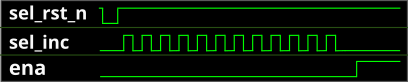
\includegraphics[width=0.75\textwidth]{./Figure/ProjectSelection.png}
  \caption{Project Selection}
  \label{fig:TINYTAPEOUTPROJECTSELECTION}
\end{figure}
%----------------------------------

%==============================================================
\section{Design flow of Tiny Tapeout}
%--------------------------------------------------------------
This section briefly describes the design flow supported by Tiny Tapeout for logic ICs designed using RTL description.

For RTL-based logic IC design, Libre Lane, shown in Figure~\ref{fig:TINYTAPEOUTLIBRELANE}, is used. Libre Lane executes the following series of steps, from RTL to layout, in a single pass. This is an approach nearly as simple as working with an FPGA.

\begin{enumerate}
  \item Logic synthesis of the RTL description
  \item Timing verification with estimated (virtual) load
  \item Automatic place and route
  \item Timing verification with actual load
  \item Generation of layout GDS data
  \item DRC/LVS verification
\end{enumerate}

%----------------------------------
\begin{figure}[htbp]
  \centering
  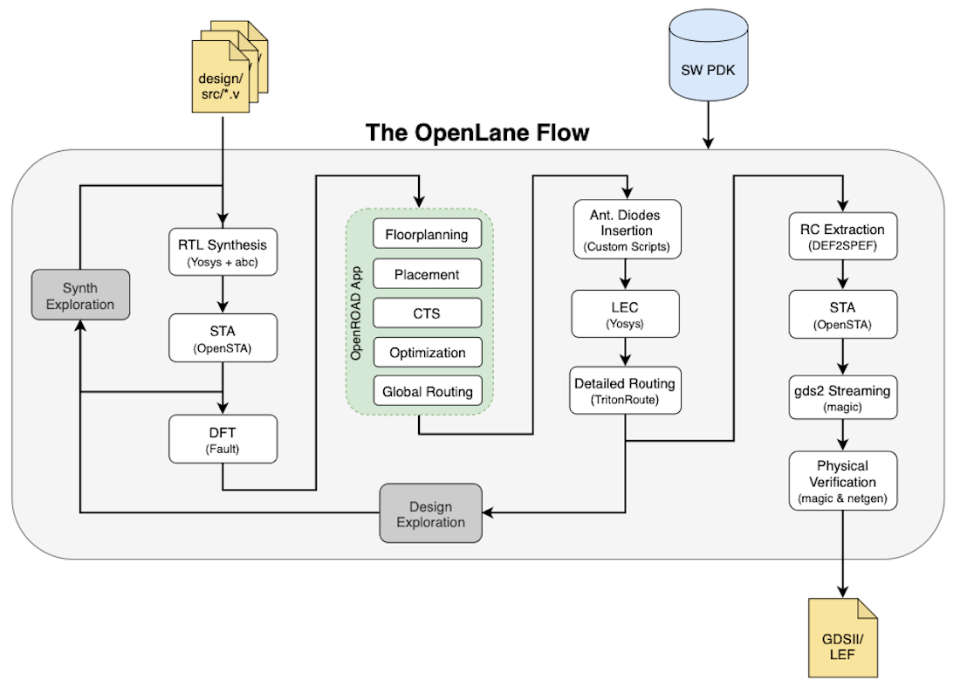
\includegraphics[width=1.0\textwidth]{./Figure/LibreLane.png}
  \caption{Design Flow of Tiny Tapeout; LibreLane (\url{https://www.zerotoasiccourse.com/terminology/librelane/})}
  \label{fig:TINYTAPEOUTLIBRELANE}
\end{figure}
%----------------------------------

As the logic verification environment for Tiny Tapeout, cocotb (Coroutine Cosimulation Testbench), shown in Figure~\ref{fig:TINYTAPEOUTCOCOTB}, is used. This allows sophisticated testbenches to be written in Python. Icarus Verilog is used as the logic simulator, interfacing with Python via the GPI (Generic Procedural Interface); various commercial logic simulators are also supported.

%----------------------------------
\begin{figure}[htbp]
  \centering
  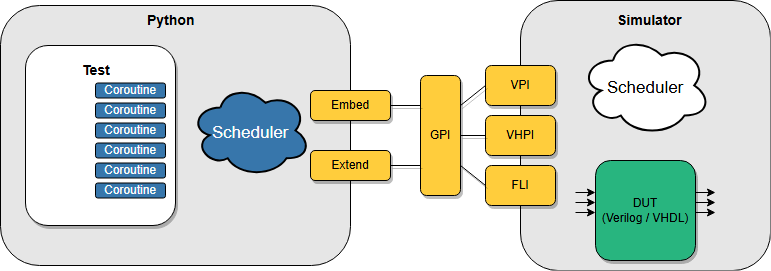
\includegraphics[width=1.0\textwidth]{./Figure/cocotb.png}
  \caption{Test Bench for Logic Verification; cocotb (\url{https://docs.cocotb.org/en/stable/index.html})}
  \label{fig:TINYTAPEOUTCOCOTB}
\end{figure}
%----------------------------------

For details on how to set up the Tiny Tapeout design environment and how to carry out actual chip design, please refer to the Tiny Tapeout website (\url{https://tinytapeout.com/}) and its GitHub repository (\url{https://github.com/TinyTapeout/}).

%==============================================================
\section{Top Level RTL of MCS4\_CPU}
%--------------------------------------------------------------
In Figure~\ref{fig:TINYTAPEOUTCONNECITON}, the connection method between the chip MCS4\_CPU created with Tiny Tapeout and the system MCS4\_SYS built on an FPGA is shown. To prevent device damage in the event of signal contention, the data bus shall be open-drain (with pull-up resistors). \\
The FPGA on the MCS4\_SYS side does have an input pull-up resistor, but its value is as large as 20\,k$\Omega$ to 100\,k$\Omega$, which can result in a long transition time to the High level. It is recommended to add an external pull-up resistor of roughly a few k$\Omega$ to 10\,k$\Omega$ on the data bus wiring outside the chip.

%----------------------------------
\begin{figure}[htbp]
  \centering
  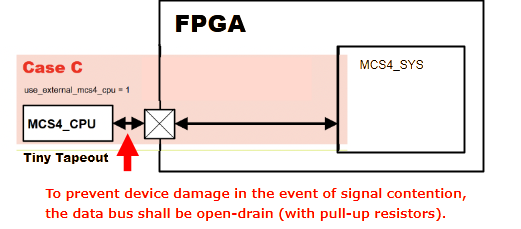
\includegraphics[width=0.75\textwidth]{./Figure/Connection.png}
  \caption{Connection of Tiny Tapeout Chip (MCS4\_CPU) and FPGA System (MCS4\_SYS)}
  \label{fig:TINYTAPEOUTCONNECITON}
\end{figure}
%----------------------------------

The RTL code of top layer of Tiny Tapeout chip (tt\_um\_mcs4\_cpu.v) is shown in Listing~\ref{list:TOPRTL}.
\\
%----------------------------------
\begin{lstlisting}[caption=tt\_um\_mcs4\_cpu.v, 
label=list:TOPRTL, captionpos=b,  language=, frame=single, basicstyle=\ttfamily\scriptsize, breaklines=true, breakatwhitespace=true]
`default_nettype none

//======================================
// Module : MCS-4 4004 CPU Chip
//======================================
module tt_um_mcs4_cpu
(
    input  wire [7:0] ui_in,    // Dedicated inputs
    output wire [7:0] uo_out,   // Dedicated outputs
    input  wire [7:0] uio_in,   // IOs: Input path
    output wire [7:0] uio_out,  // IOs: Output path
    output wire [7:0] uio_oe,   // IOs: Enable path (active high: 0=input, 1=output)
    input  wire       ena,      // always 1 when the design is powered, so you can ignore it
    input  wire       clk,      // clock
    input  wire       rst_n     // reset_n - low to reset
);

integer i;

//---------------------
// Interface Signals
//---------------------
wire        sync_n;   // Sync Signal
wire [ 3:0] data_o;   // Data Output
wire        data_oe;  // Data Output Enable
wire [ 3:0] data_i;   // Data Input
wire        cm_rom_n; // Memory Control for ROM
wire [ 3:0] cm_ram_n; // Memory Control for RAM
wire        test;     // Test Input

//---------------------
// I/O Connection
//---------------------
assign test       = ui_in[0];
assign uo_out[0]  = sync_n;
assign uo_out[1]  = cm_rom_n;
assign uo_out[2]  = 1'b0;
assign uo_out[3]  = 1'b0;
assign uo_out[4]  = cm_ram_n[0];
assign uo_out[5]  = cm_ram_n[1];
assign uo_out[6]  = cm_ram_n[2];
assign uo_out[7]  = cm_ram_n[3];
assign data_i[0]  = uio_in[0];
assign data_i[1]  = uio_in[1];
assign data_i[2]  = uio_in[2];
assign data_i[3]  = uio_in[3];
assign uio_out[0] = 1'b0; // open drain
assign uio_out[1] = 1'b0; // open drain
assign uio_out[2] = 1'b0; // open drain
assign uio_out[3] = 1'b0; // open drain
assign uio_out[4] = 1'b0;
assign uio_out[5] = 1'b0;
assign uio_out[6] = 1'b0;
assign uio_out[7] = 1'b0;
assign uio_oe[0]  = data_oe & ~data_o[0]; // open drain
assign uio_oe[1]  = data_oe & ~data_o[1]; // open drain
assign uio_oe[2]  = data_oe & ~data_o[2]; // open drain
assign uio_oe[3]  = data_oe & ~data_o[3]; // open drain
assign uio_oe[4] = 1'b0;
assign uio_oe[5] = 1'b0;
assign uio_oe[6] = 1'b0;
assign uio_oe[7] = 1'b0;

// List all unused inputs to prevent warnings
wire _unused = &{ena, uio_in[7:4], 1'b0};

//--------------------
// MCS-4 4004 CPU Core
//--------------------
MCS4_CPU U_MCS4_CPU
(
    .CLK   (clk),      // clock
    .RES_N (rst_n),    // reset_n
    //
    .SYNC_N   (sync_n),   // Sync Signal
    .DATA_I   (data_i),   // Data Input
    .DATA_O   (data_o),   // Data Output
    .DATA_OE  (data_oe),  // Data Output Enable
    .CM_ROM_N (cm_rom_n), // Memory Control for ROM
    .CM_RAM_N (cm_ram_n), // Memory Control for RAM
    .TEST     (test)      // Test Input
);

endmodule
\end{lstlisting}
%----------------------------------


 %==============================================================
\section{Project Information file for Tiny Tapeout}
%--------------------------------------------------------------
 We should modify the project information info.yaml as shown in Listing~\ref{list:INFOYAML}. This file specify tile size, top module name, RTL file names and usage of I/O pins.
\\ 
%----------------------------------
\begin{lstlisting}[caption=info.yaml, 
label=list:INFOYAML, captionpos=b,  language=, frame=single, basicstyle=\ttfamily\scriptsize, breaklines=true, breakatwhitespace=true]
# Tiny Tapeout project information
project:
  title:        "MCS-4 4004 CPU"      # Project title
  author:       "Munetomo Maruyama"   # Your name
  discord:      "munetomo_85572"      # Your discord username, for communication and automatically assigning you a Tapeout role (optional)
  description:  "MCS-4 4004 CPU"      # One line description of what your project does
  language:     "Verilog"    # other examples include SystemVerilog, Amaranth, VHDL, etc
  clock_hz:     750000       # Clock frequency in Hz (or 0 if not applicable)

  # How many tiles your design occupies? A single tile is about 167x108 uM.
  tiles: "1x1"          # Valid values: 1x1, 1x2, 2x2, 3x2, 4x2, 6x2 or 8x2

  # Your top module name must start with "tt_um_". Make it unique by including your github username:
  top_module:  "tt_um_mcs4_cpu"

  # List your project's source files here.
  # Source files must be in ./src and you must list each source file separately, one per line.
  # Don't forget to also update `PROJECT_SOURCES` in test/Makefile.
  source_files:
    - "tt_um_mcs4_cpu.v"
    - "mcs4_cpu.v"
    
  # The pinout of your project. Leave unused pins blank. DO NOT delete or add any pins.
  # This section is for the datasheet/website. Use descriptive names (e.g., RX, TX, MOSI, SCL, SEG_A, etc.).
pinout:
  # Inputs
  ui[0]: "TEST"
  ui[1]: ""
  ui[2]: ""
  ui[3]: ""
  ui[4]: ""
  ui[5]: ""
  ui[6]: ""
  ui[7]: ""

  # Outputs
  uo[0]: "SYNC_N"
  uo[1]: "CM_ROM_N"
  uo[2]: ""
  uo[3]: ""
  uo[4]: "CM_RAM_N[0]"
  uo[5]: "CM_RAM_N[1]"
  uo[6]: "CM_RAM_N[2]"
  uo[7]: "CM_RAM_N[3]"

  # Bidirectional pins
  uio[0]: "DATA[0]"
  uio[1]: "DATA[1]"
  uio[2]: "DATA[2]"
  uio[3]: "DATA[3]"
  uio[4]: ""
  uio[5]: ""
  uio[6]: ""
  uio[7]: ""

# Do not change!
yaml_version: 6
\end{lstlisting}
%----------------------------------

 %==============================================================
\section{Layout Design of MCS4\_CPU and its Assignment in the Chip}
%--------------------------------------------------------------
The Tiny Tapeout repository of this project is \url{https://github.com/munetomo-maruyama/ttsky25a_MCS4_CPU}.\\
The layout data (GDS-II) of  MCS4\_CPU is shown in Figure~\ref{fig:TINYTAPEOUTLAYOUT}, and its assignment position in the chip is shown in Figure~\ref{fig:TINYTAPEOUTASSIGNMENT}.

%----------------------------------
\begin{figure}[htbp]
  \centering
  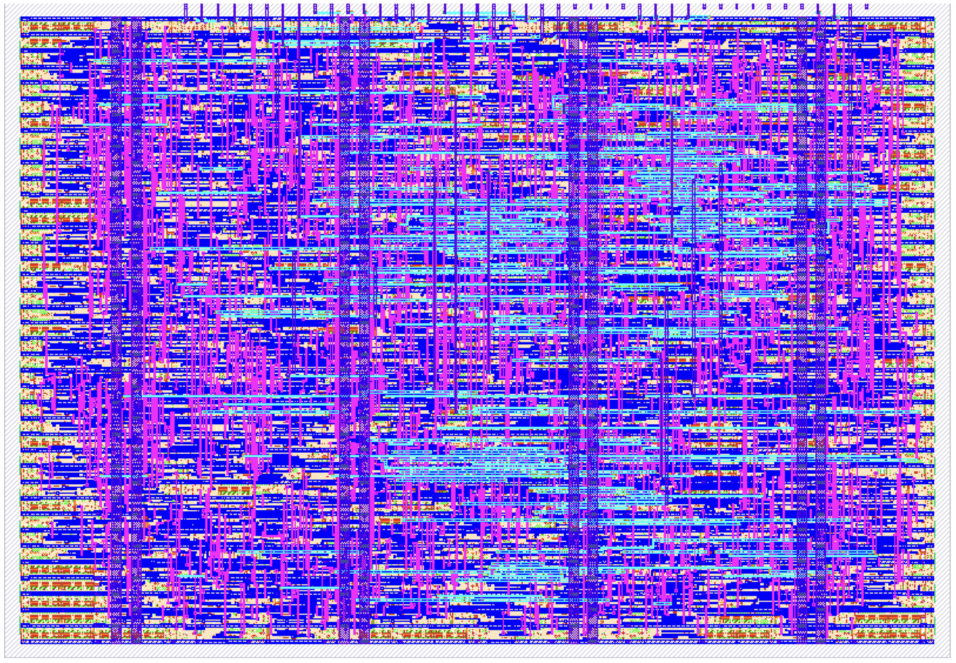
\includegraphics[width=1.0\textwidth]{./Figure/Layout.png}
  \caption{Layout Design of MCS4\_CPU}
  \label{fig:TINYTAPEOUTLAYOUT}
\end{figure}
%----------------------------------
%----------------------------------
\begin{figure}[htbp]
  \centering
  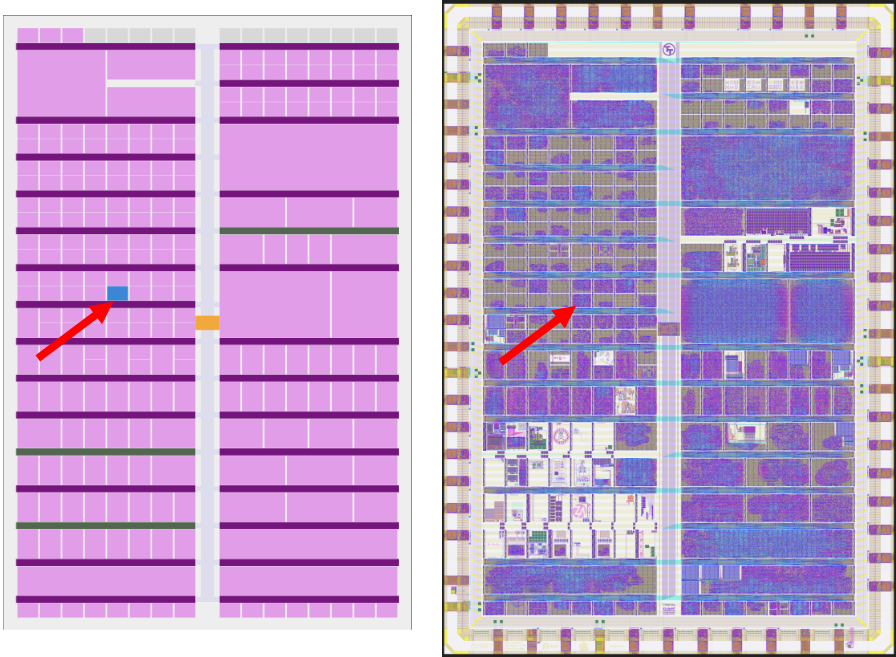
\includegraphics[width=0.75\textwidth]{./Figure/Assignment.png}
  \caption{Assignment in the Chip}
  \label{fig:TINYTAPEOUTASSIGNMENT}
\end{figure}
%----------------------------------

 %==============================================================
\section{Debugging}
%--------------------------------------------------------------
The chip prototyped through Tiny Tapeout is mounted on a breakout board and delivered together with a demo board (ETR). The demo board (ETR) carries an RP2040 microcontroller, which can select the project on the Tiny Tapeout chip and, if needed, supply the clock and reset and control the user input/output signals. For details, please refer to \url{https://tinytapeout.com/guides/get-started-demoboard-etr/}. As a result, the MCS4\_CPU worked perfectly.

%----------------------------------
\begin{figure}[htbp]
  \centering
  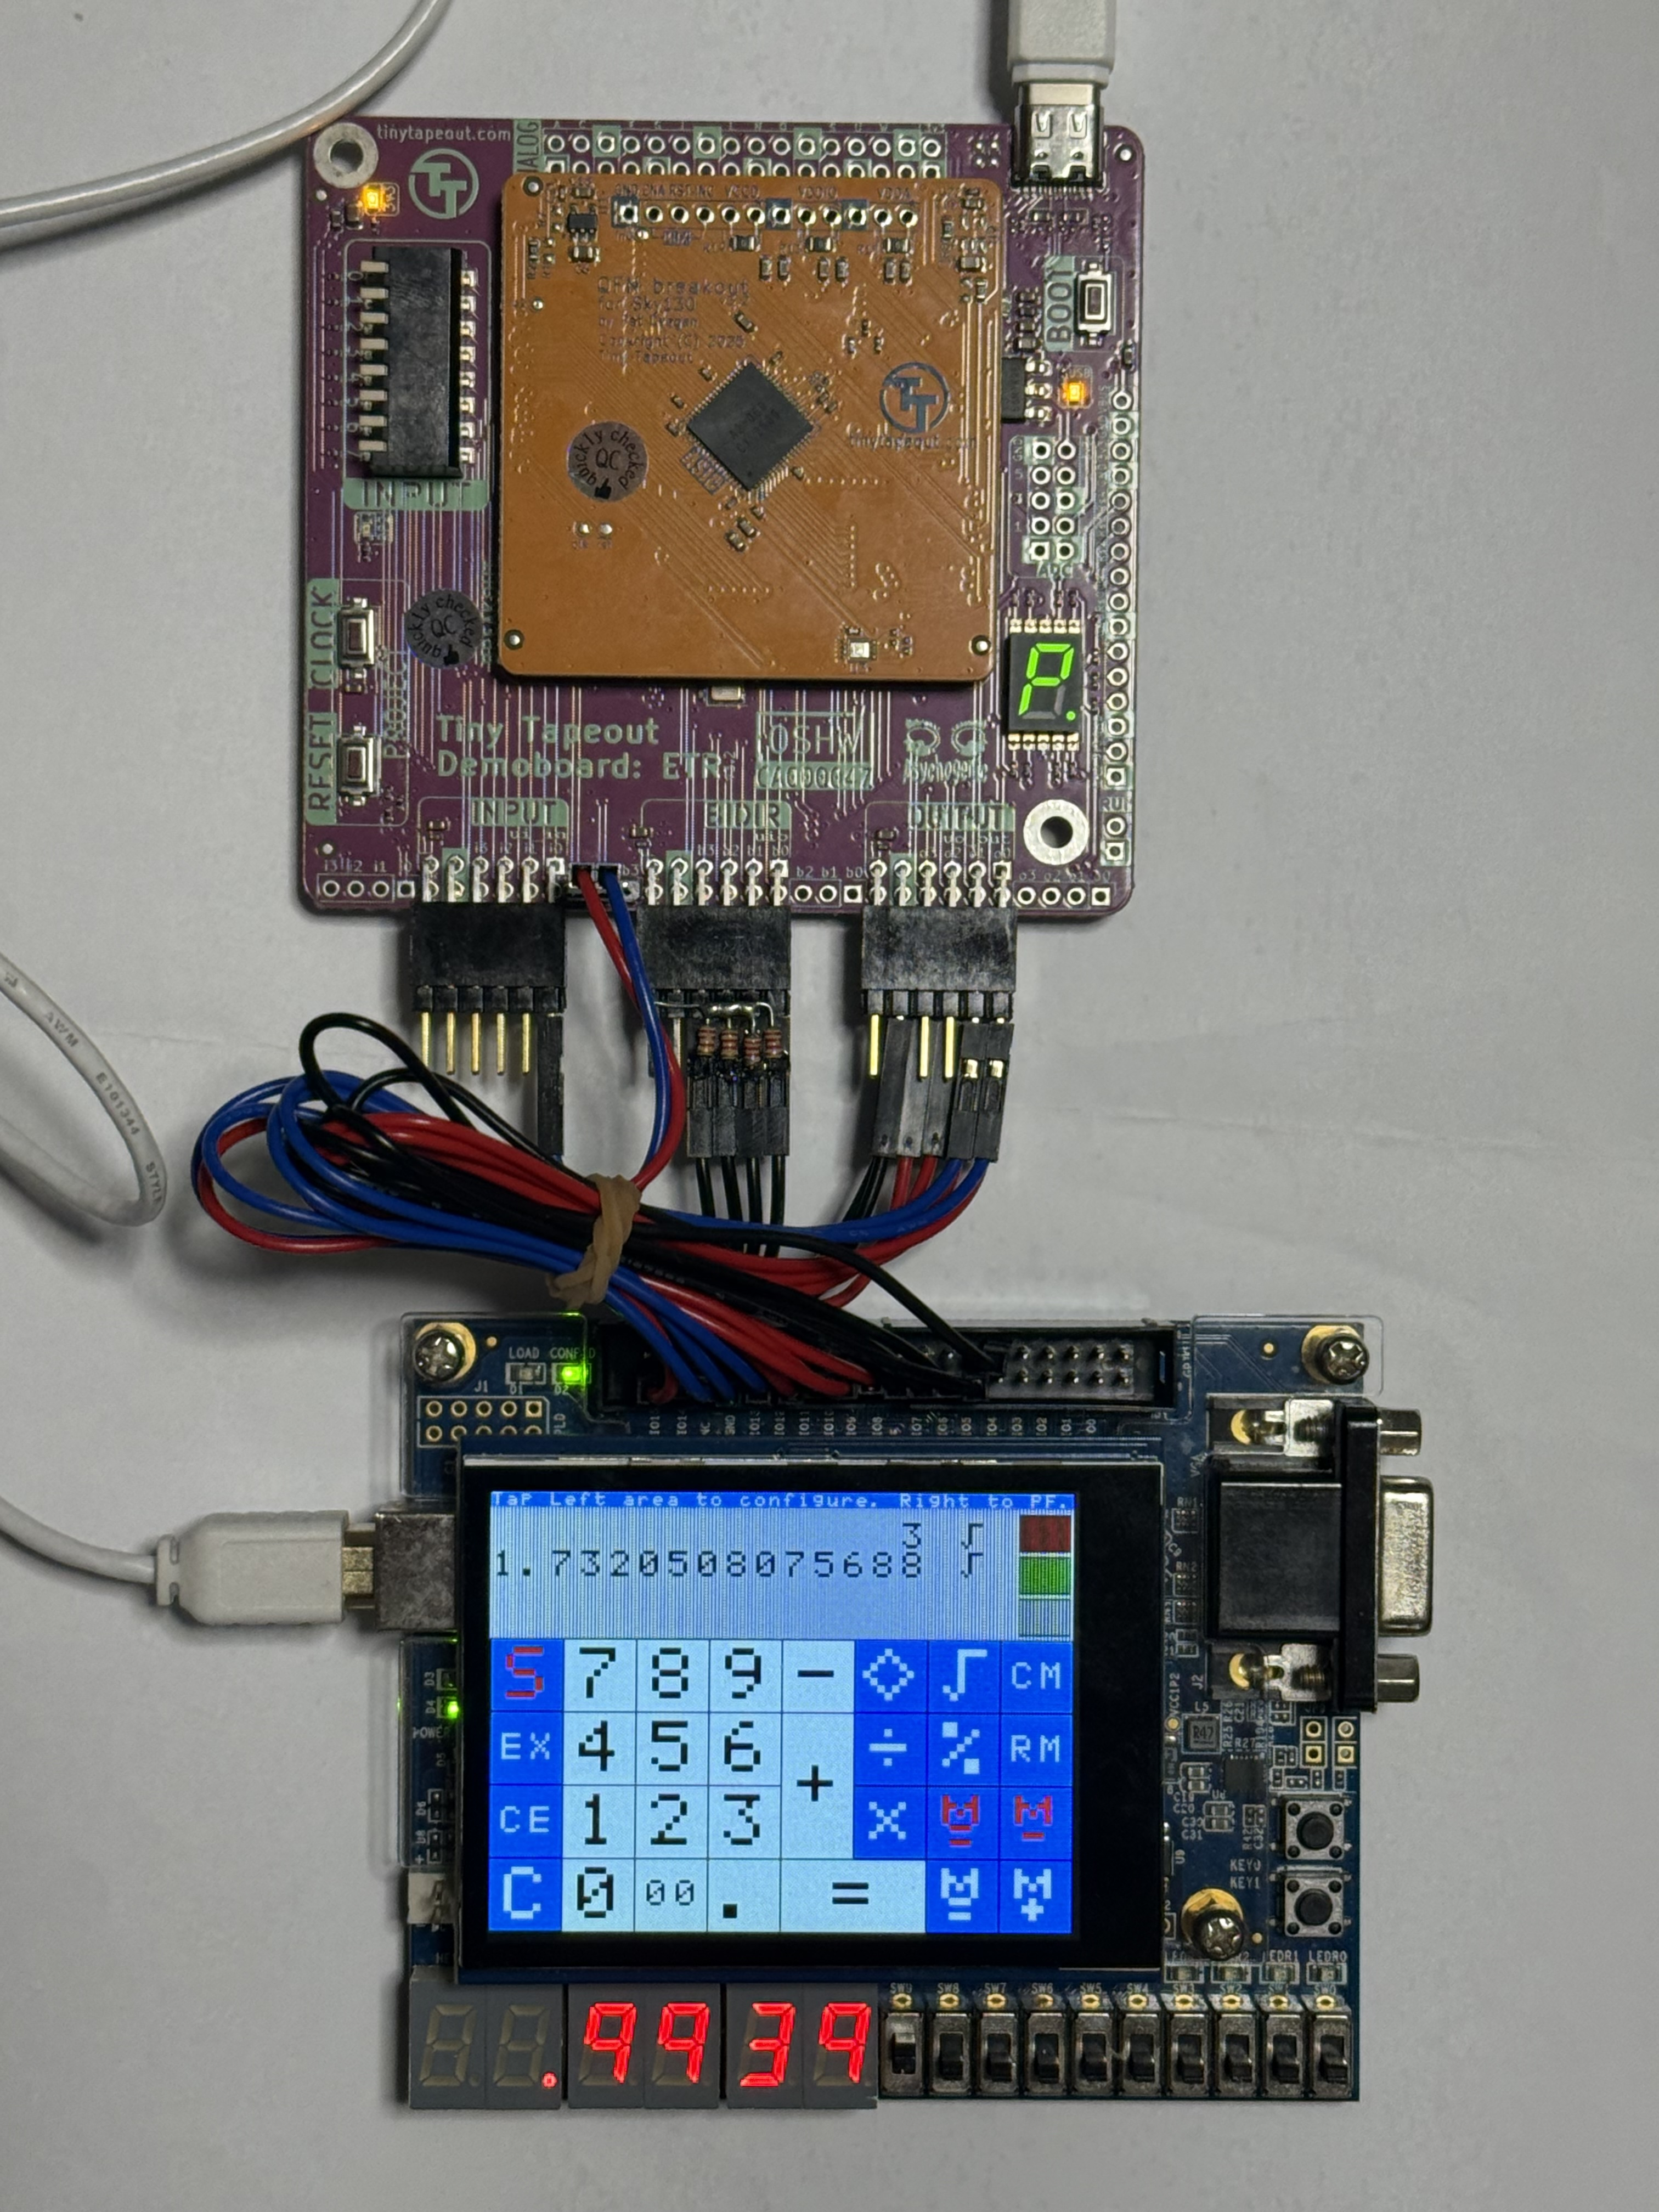
\includegraphics[width=0.5\textwidth]{./Figure/Debug.jpg}
  \caption{Worked perfectry!}
  \label{fig:TINYTAPEOUTDEBUG}
\end{figure}
%----------------------------------

%===================================================
\subsubsection*{Notes on Hold Timing Issue}
%---------------------------------------------------
This entire system employs synchronous design referenced to the rising edge of a single-phase clock, which is common practice in RTL design. As long as this remains within a single chip, clock skew is aligned and timing verification passes, so there is no problem. On the other hand, a problem can arise when MCS4\_CPU and MCS4\_SYS are physically implemented as separate chips. Even when implemented as separate chips, operation may still be possible if both are FPGAs of the same process and the same series. However, since the Tiny Tapeout chip corresponding to MCS4\_CPU is fabricated in a 130\,nm process, while the FPGA corresponding to MCS4\_SYS, an Altera MAX~10, uses a 55\,nm process, there is essentially no case in which the clock skew between the two matches. In such cases, what can become a problem is a violation of the setup time and hold time of the D flip-flops. However, since this system operates at a slow clock frequency of 750\,MHz, setup time is essentially never an issue. The problem is hold time violation.

\begin{enumerate}
\item \textbf{CPU output control signals}

Figure~\ref{fig:TINYTAPEOUTHOLDISSUE01}(a) shows the timing of the MCS4\_CPU output control signals relative to the CPU clock C\_CLK. Here, it is assumed that the signals are output with zero delay.

Figure~\ref{fig:TINYTAPEOUTHOLDISSUE01}(b) shows the behavior on the MCS4\_SYS side that receives these signals. Here, it is assumed that the SYS clock S\_CLK lags slightly behind the CPU clock C\_CLK. In this case, when the MCS4\_SYS side captures the MCS4\_CPU output control signals, the hold time cannot be guaranteed, and there is a possibility that the signals cannot be correctly transferred.

Figure~\ref{fig:TINYTAPEOUTHOLDISSUE01}(c) shows the countermeasure for this. On the MCS4\_SYS side, a clock S\_CLK\_F, whose phase is advanced slightly relative to the SYS clock S\_CLK, is generated, and the CPU output control signals are first captured using this clock. If these are then captured again by the internal SYS clock S\_CLK of MCS4\_SYS, no hold violation occurs.

%----------------------------------
\begin{figure}[htbp]
  \centering
  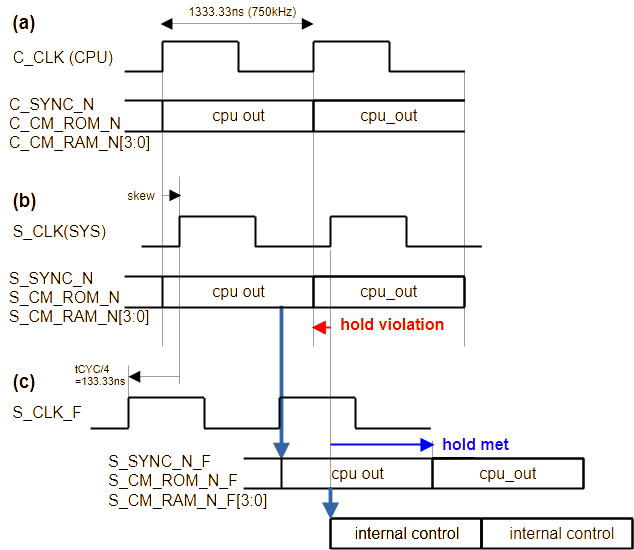
\includegraphics[width=0.5\textwidth]{./Figure/HoldIssue01.png}
  \caption{Hold Timing Issue (1)}
  \label{fig:TINYTAPEOUTHOLDISSUE01}
\end{figure}
%----------------------------------

\item \textbf{Bidirectional data bus (DATA) during CPU output (address output, write data output)}

Figure~\ref{fig:TINYTAPEOUTHOLDISSUE02}(a) shows the timing of the MCS4\_CPU data bus output relative to the CPU clock C\_CLK. Here, it is assumed that the signals are output with zero delay.

Figure~\ref{fig:TINYTAPEOUTHOLDISSUE02}(b) shows the behavior on the MCS4\_SYS side that receives these signals. Here, it is assumed that the SYS clock S\_CLK lags slightly behind the CPU clock C\_CLK. In this case, when the MCS4\_SYS side captures the MCS4\_CPU data bus output, the hold time cannot be guaranteed, and there is a possibility that the signals cannot be correctly transferred.

Figure~\ref{fig:TINYTAPEOUTHOLDISSUE02}(c) shows the countermeasure for this. On the MCS4\_SYS side, a clock S\_CLK\_F, whose phase is advanced slightly relative to the SYS clock S\_CLK, is generated, and the CPU data bus output is first captured using this clock. If it is then captured again by the internal SYS clock S\_CLK of MCS4\_SYS, no hold violation occurs.

The following discusses the capture, on the SYS side, of the CPU-side output from the data bus, together with the switching of the data bus direction.

\begin{itemize}
\item In CPU states A1, A2, and A3, the CPU outputs the address, and in the following states M1 and M2, the CPU inputs the instruction code. The direction of the data bus changes between state A3 and state M1; however, just before this change, the MCS4\_SYS side has already captured the CPU address output of state A3 using clock S\_CLK\_F, so no hold violation occurs and there is no problem.
\item There is an instruction in which the CPU outputs write data in CPU state X2, and if nothing is placed on the data bus in the states immediately before and after it, the capture on the MCS4\_SYS side in state X2 is performed without any hold violation.
\item When the CPU outputs write data in CPU states X2 and X3, the address is also output continuously in the following state A1. In this case as well, the capture on the MCS4\_SYS side is performed without any hold violation.
\end{itemize}

%----------------------------------
\begin{figure}[htbp]
  \centering
  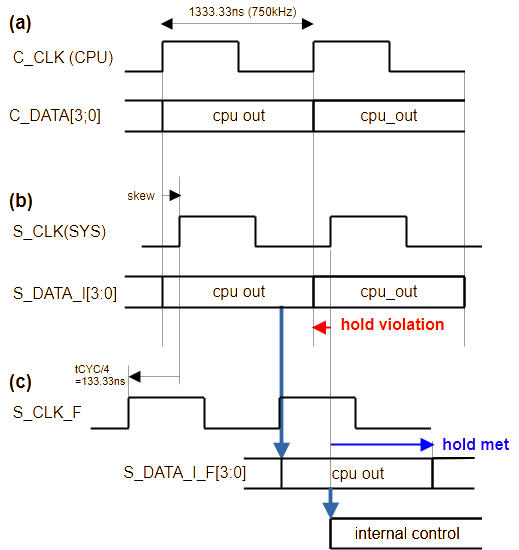
\includegraphics[width=0.5\textwidth]{./Figure/HoldIssue02.png}
  \caption{Hold Timing Issue (2)}
  \label{fig:TINYTAPEOUTHOLDISSUE02}
\end{figure}
%----------------------------------

\item \textbf{Bidirectional data bus (DATA) during CPU input (instruction code input, read data input)}

Figure~\ref{fig:TINYTAPEOUTHOLDISSUE03}(a) shows the timing of the MCS4\_SYS data bus output relative to the SYS clock S\_CLK. Here, it is assumed that the signals are output with zero delay, and that the SYS clock S\_CLK is slightly advanced relative to the CPU clock C\_CLK.

Figure~\ref{fig:TINYTAPEOUTHOLDISSUE03}(b) shows the behavior on the MCS4\_CPU side that receives this signal. In this case, when the MCS4\_CPU side captures the MCS4\_SYS data bus output, the hold time cannot be guaranteed, and there is a possibility that the signal cannot be correctly transferred.

Figure~\ref{fig:TINYTAPEOUTHOLDISSUE03}(c) shows the countermeasure for this. On the MCS4\_SYS side, a clock S\_CLK\_B, whose phase is delayed slightly relative to the SYS clock S\_CLK, is generated, and output from the data bus is performed at this timing. If this is captured by the internal CPU clock C\_CLK of MCS4\_CPU, no hold violation occurs.

The following discusses the capture, on the CPU side, of the SYS-side output from the data bus, together with the switching of the data bus direction.

\begin{itemize}
\item In CPU states A1, A2, and A3, the CPU outputs the address, and in the following states M1 and M2, the CPU inputs the instruction code. In state X1, which follows state M2, no one drives the data bus, so the data bus is pulled up to a High level by the pull-up resistor. The data output from SYS in states M1 and M2 is delayed relative to the CPU side, and as long as there is also a delay in the High transition due to the pull-up resistor, no hold violation occurs on the CPU side.
\item There is an instruction in which the CPU inputs read data in CPU state X2, and in the states immediately before and after it, no one drives the data bus. While it is not driven, the data bus is pulled up to a High level by the pull-up resistor. The data output from SYS in state X2 is delayed relative to the CPU side, and as long as there is also a delay in the High transition due to the pull-up resistor, no hold violation occurs on the CPU side.
\end{itemize}
\end{enumerate}

%----------------------------------
\begin{figure}[htbp]
  \centering
  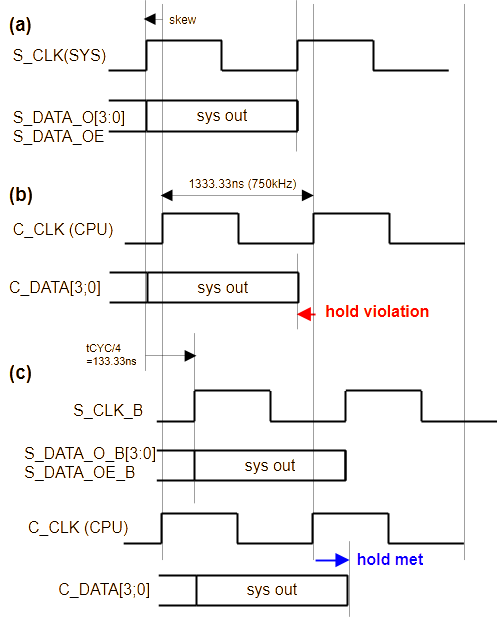
\includegraphics[width=0.5\textwidth]{./Figure/HoldIssue03.png}
  \caption{Hold Timing Issue (3)}
  \label{fig:TINYTAPEOUTHOLDISSUE03}
\end{figure}
%----------------------------------

%==============================================================
